\documentclass[tikz]{standalone}
\usepackage{fontspec}
\renewcommand*{\familydefault}{\sfdefault}
\usepackage{standalone}
\usepackage{amssymb}
\usetikzlibrary{decorations}
\usetikzlibrary{arrows.meta, decorations.pathmorphing, decorations.pathreplacing, shapes.geometric}
\usetikzlibrary{bayesnet}

\begin{document}

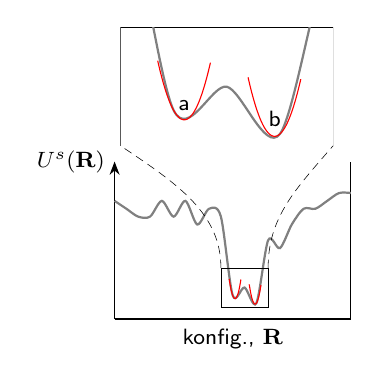
\begin{tikzpicture}[font=\footnotesize, xscale=1.5]

% axes
\draw[-Stealth] (-1,0) -- (-1,2) node[anchor=east] {\(U^s(\mathbf{R})\)} ;
\draw (1,0) -- (1,2) ;
\draw (-1,0) -- node[anchor=north] {konfig.,~\(\mathbf{R}\)} (1,0) ;

% energy landscape
\draw[gray, thick] plot[smooth] coordinates {
(-1.0,1.5) (-0.9,1.4) (-0.8,1.3) (-0.7,1.3) (-0.6,1.5) (-0.5,1.3) (-0.4,1.5)
(-0.3,1.2) (-0.2,1.4) (-0.1,1.3) (0.0,0.3) (0.1,0.4) (0.2,0.2) (0.3,1.0) (0.4,0.9) (0.5,1.2) (0.6,1.4) (0.7,1.4) (0.8,1.5) (0.9,1.6) (1.0,1.6)
};

% harmonic potentials approximating landscape
\path[red, draw, domain=-0.03:0.07, samples=101] plot (\x, {pow(10 * (\x - 0.02), 2) + 0.26}) ;
\path[red, draw, domain=0.14:0.24, samples=101] plot (\x, {pow(10 * (\x - 0.19), 2)
+ 0.19}) ;

% region of interest
\draw[very thin] (-0.10,0.15) coordinate (roiLB) rectangle (0.30,0.65) coordinate (roiRT) ;


% MAGNIFIED DETAIL
\begin{scope}[xshift=-0.5 cm, yshift=+1.75 cm, xscale=4.5, yscale=3]

% region of interest
\clip (-0.10,0.15) coordinate (zoomLB) rectangle (0.30,0.65) coordinate (zoomRT) ;

% region of interest
\draw[very thin] (-0.10,0.15) rectangle (0.30,0.65) ;

% energy landscape
\draw[gray, thick] plot[smooth] coordinates {
(-1.0,1.5) (-0.9,1.4) (-0.8,1.3) (-0.7,1.3) (-0.6,1.5) (-0.5,1.3) (-0.4,1.5)
(-0.3,1.2) (-0.2,1.4) (-0.1,1.3) (0.0,0.3) (0.1,0.4) (0.2,0.2) (0.3,1.0) (0.4,0.9) (0.5,1.2) (0.6,1.4) (0.7,1.4) (0.8,1.5) (0.9,1.6) (1.0,1.6)
};

% harmonic potentials approximating landscape
\path[red, draw, domain=-0.03:0.07, samples=101] plot (\x, {pow(10 * (\x - 0.02), 2) + 0.26}) ;
\path[red, draw, domain=0.14:0.24, samples=101] plot (\x, {pow(10 * (\x - 0.19), 2)
+ 0.19}) ;

% label basins
\path
(+0.02,0.26) node[anchor=south] {a}
(+0.19,0.19) node[anchor=south] {b}
;

\end{scope}

\draw[very thin, densely dashed]
(roiLB |- roiRT) to[out=90, in=-45] (zoomLB)
(roiRT) to[out=90, in=-120] (zoomLB -| zoomRT)
;

\end{tikzpicture}

\end{document}


